\documentclass[conference]{IEEEtran}
\IEEEoverridecommandlockouts
% The preceding line is only needed to identify funding in the first footnote. If that is unneeded, please comment it out.
\usepackage{url}
\usepackage{cite}
\usepackage{amsmath,amssymb,amsfonts}
\usepackage{algorithmic}
\usepackage{graphicx}
\usepackage{textcomp}
\usepackage{algorithm2e}
\usepackage{xcolor}
\def\BibTeX{{\rm B\kern-.05em{\sc i\kern-.025em b}\kern-.08em
    T\kern-.1667em\lower.7ex\hbox{E}\kern-.125emX}}
\begin{document}

\title{
  What should I notice? Evaluating unexpectedness of events to generate surprising causal candidates.
}
\author{
  \IEEEauthorblockN{
  \IEEEauthorrefmark{1}\IEEEauthorrefmark{2} Étienne Houzé,
  \IEEEauthorrefmark{1} Jean-Louis Dessalles,
  \IEEEauthorrefmark{1} Ada Diaconescu,
  \IEEEauthorrefmark{2} David Menga
  }

  \IEEEauthorblockA{\IEEEauthorrefmark{1}
    Télécom Paris, IP Paris, \emph{Palaiseau}, France\\
  email: \{first\}.\{second\}@telecom-paris.fr}
  \IEEEauthorblockA{\IEEEauthorrefmark{2} EDF R\&{}D, \emph{Palaiseau}, France\\
  email: \{first\}.\{second\}@edf.fr}
}

\maketitle

\begin{abstract}
  When confronted to an unprecedented situation, humans typically show good performance in quickly identifying noticeable past events and proposing them as possible causal hypotheses. Our research focuses on emulating this behaviour into devices, as to deal with rare, unusual situations where previously acquired knowledge fails to provide hypotheses. We rely on a definition of the unexpectedness of events based on Algorithmic Information Theory and the notion of Kolmogorov Complexity. We illustrate our proposal on a simulated smart homes undergoing various unusual events over the course of more than a year.
\end{abstract}

\begin{IEEEkeywords}
component, formatting, style, styling, insert
\end{IEEEkeywords}

\section{Introduction}

The ability to infer new causal relations is one of the many tasks in which humans prevail but machines still fall short of completing. This ability is prime in making discoveries, or acquiring new knowledge by making educated guesses.

Without any knowledge about how physics or electricty work, it would be possible to infer a possible link between a memorable thunderstorm and a general black-out only by using the noticeability score of the first. While this kind of abductive inference can yield many false-positives, its application can be to propose new hypotheses to be tested out when other possible methods of inference fail to provide any hypothesis (due to a lack of prior similar situations, or to the importance of the context). The difficulty of this approach to reasoning is, however, to quickly identify the relevant candidate hypotheses. In this regards, we may use a basic instinct: without prior knowledge, the most relevant hypothesis might simply be the most memorable recent event. However this definition is highly subjective, and does not seem to fit well into the canvas of computing and AI.

A possible approach would be to rely on the naming complexity of events: memorable events are more likely to be shorter to be named than boring usual events. Think, for instance, of how ``last year's hottest day'' description appears much simpler than ``the 182th day of 7 years ago''. Our idea is to rely on this metrics to estimate the description complexity of events. Then, by comparing the description complexity of a given event $e$ to the average complexity of similar events, we induce a measure of unexpectedness that can be used to assess the most memorable events.

\begin{figure}[ht]
  \centering
  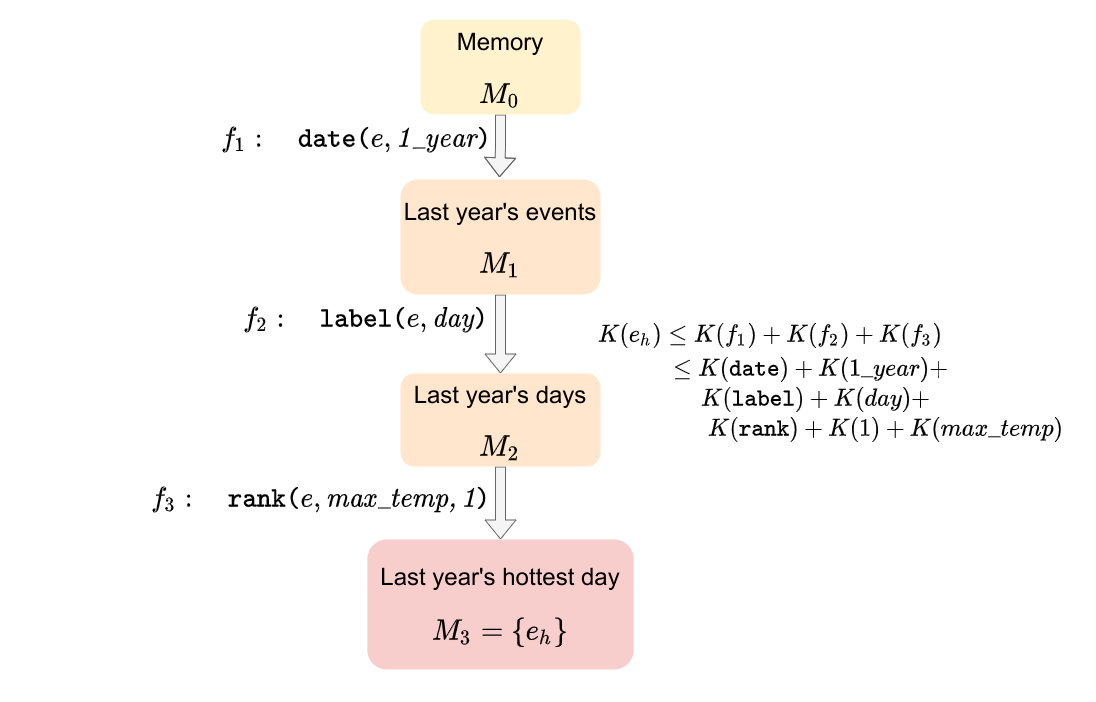
\includegraphics[width=\linewidth]{figures/filters}
  \caption{An example of retrieving an event through successive predicative filters. The ``hottest day of last year'' is accessed by selecting day-type events, from last year, and looking for the one ranked first by maximum temperature.}
  \label{fig:filters}
\end{figure}

To programatically achieve what humans are easily capable to do, we rely on a basic model intuition of how memory works. We assume that a memory is a unordered set of various distinct objects, upon which can be applied boolean predicates to describe them. These predicates thus provide filters that can be applied to the memory. By applying successive filters, we narrow down the size of the memory, until a single event remains. The complexity of this remaining events can thus be estimated as the simplest combination of predicative filter that uniquely describe it.

The rest of this paper is as follows: we first briefly introduce some notions of Algorithmic Information Theory and its applications in section \ref{sec:theory}, then we explicit our methods of computing the unnexpectedness of past events in cyber-physical systems \ref{sec:computing}. We illustrate this approach by providing an implementation relying on a few predicates on events from a smart home simulation \ref{sec:example}. In section \ref{sec:related} we briefly review other related works using complexity theory or trying to explain smart homes and how our work can be linked with them.

\section{Theoretical Background}
\label{sec:theory}
The notion of complexity formally quantifies the amount of information required for the computation of a binary string (or any object representable by a finite bynary string)\cite{kolmogorov_three_1965,li_introduction_2008}. For such a binary string $s$, its complexity $K(s)$, is the bit length of the shortest program $p$ which, if given as input to a universal Turing Machine $U$, outputs $s$.
\begin{equation}
  K_{U}(s) = \min_{p}\left\{l(p)|U(p)=s\right\}
\end{equation}
The first notable property of this definition is its universality: given that a Turing machine $U'$ can be encoded into $U$ using a program $p_{U}$, we have the following inequality:
\begin{equation}
  K_{U}(s) \le l(p_{u}) + K_{U}(s)
\end{equation}
since the additional constant does not depend on the string $s$, we can drop the requirement on a given machine $U$ and use a universal complexity $K(s)$, such that:
\begin{equation}
  \forall U\in\text{TM}, \forall s, |K(s) - K_{u}(s)| \le C_{U}
\end{equation}
It is important to note that the notion of Kolmogorov complexity is not related to the computation complexity, as there is no requirement on the execution time of the programs, only their length in bits matters for the computation of complexity. In fact, it can be shown that Kolmogorov complexity is not computable\cite{li_introduction_2008}. The sketch of the proof is that computing the Kolmogorov complexity would require to run all programs, up to a certain length, which includes non-terminating ones. As the termination of programs is non-decidable, the computation of complexity is not.

While the introducion of Kolmogorov complexity was purely theoretical, many applications were found, notably because of its close relation with the intuitive notions of the complexity of items, events, situations. For instance,~\cite{murena_solving_2020} studied the use of Kolmogorov Complexity to identify and solve analogies.

Algorithmic Information Theory is also used to define the notion of unexpectedness: in \cite{dessalles2011coincidences}, the unexpectedness $U(e)$ of an event is defined as the difference between an a-priori expected causal complexity $C_{w}(e)$ and the actual observed complexity $C(e)$
\begin{equation}
  \label{eq:unexpected}
  U(e) = |C_{w}(e) - C(e)|
\end{equation}
Using this measure, it is possible to model phenomenons such as coincidences: imagine that you happen to run into a friend in a park. The unnexpectedness will be much larger if this park is in Singapore than if it is in your common neighbourhood: the causal complexity $C_{w}$ is much higher if you a priori have no knowledge of your friend being around, while the description complexity remains the same.

\section{Computing the unexpectedness of events}
\label{sec:computing}
\subsection{A memory model}
We model the memory as an unordered set $M$ of events $e$. Individual events can be seen as data points, augmented with a label indicating their nature (temperature events, failure events, addition/removal events), and a timestamp:
\begin{equation}
  e \equiv (l, t,\mathcal{D})
\end{equation}
where $l$ is the label, $t$ a timestamp and $\mathcal{D}$ a multi-dimensional datapoint representing various characteristics of the events (e.g.~its duration, the maximum temperature reached, the sensor name, its position).

We define \emph{predicates} as boolean function operating on these events, and taking an additional argument, encoded as a finite binary string
\begin{equation}
  \pi : \begin{cases}
    \mathcal{M}\times \{0,1\}^{*} &\mapsto \{0,1\} \\
    (e, k) &\mapsto \pi_{k}(e)
    \end{cases}
\end{equation}
Using this construction allows for structures such as \emph{max\_temperature(e, T)}, where $e$ is the event argument and $T$ a temperature described by the finite binary string.

From these predicates, we can construct filter operations on the memory. A filter operates by simply selecting the events satisfying a given predicate $\pi_{k}$ and constructing a resulting memory from these events.
\begin{equation}
 f_{\pi, k}(\mathcal{M}) = \left\{e \in \mathcal{M} | \pi_{k}(e) \right\}
\end{equation}
For example, the filter ``last year'' corresponds to $\pi = \mathit{date}$ and $k = \mathtt{last year}$.

\subsection{Description complexity of events}

From the previous definitions, we then estimate the complexity of events as the ``simplest'' way of retrieving them from the memory, by applying successive filters. A retrieval path composed of various filters $p = f_{1} = f_{\pi_{1}, k_{1}}, f_{2} = f_{\pi_{2}, k_{2}}, \dots, f_{n} = f_{\pi_{n}, k_{n}}$ is said to \emph{retrieve} an event $e$ from a memory $\mathcal{M}$ if and only if $p(\mathcal{M}) = f_{1} \circ f_{2} \circ \dots \circ f_{n} (\mathcal{M}) = \{e\}$. For an event $e$, if such a path exist, its complexity can be bounded by $K(p) = \sum_{f_{\pi, k} \in p} l(\pi) + l(k)$, the complexity of the retrieval path being the sum of the bit lengths required to describe the predicates $\pi$ and their arguments $k$.

The description complexity of an event $e$ can thus be defined as the minimum complexity of a retrieval path retrieving $e$:

\begin{equation}
  \label{eq:desc_k}
  K(e) = \min_{p | p(\mathcal{M}) = e} K(p) = \min_{p | p(\mathcal{M})=e} \sum_{f_{\pi, k} \in p} l(\pi) + l(k)
\end{equation}

\subsection{Computing an unexpectedness measure}
Equation \ref{eq:unexpected} gives a universal description of unexpectedness, as the difference between the complexity of the phenomenon generating an event and the complexity required to describe this event. In our particular application case, we may directly use the description complexity $K(e)$ as defined in \ref{eq:desc_k}.

\begin{algorithm}
  \caption{Iterative computation of the complexity}
  \label{alg:complex_iter}
  $\mathtt{current_{explore}} \leftarrow [\mathcal{M}]$ \;
  $\mathtt{future_{explore} \leftarrow} [\;]$ \;
  \While{$\mathtt{current_{explore}} \neq [\;]$ \textbf{and} $\mathtt{pass} < \mathtt{max\_pass}$}{
    \For{$(\mathtt{M_{prev}}, \mathtt{K_{prev}}) \in \mathtt{current_{explore}}$}{
      \For{$\mathtt{p \in \mathcal{P}}$}{
        \For{$\mathtt{k \in \{0,1\}^{*}}$}{
          $\mathtt{K_{current} \leftarrow l(p) + l(k) + K_{prev}}$ \;
          \If{$\mathtt{K_{current}} > \mathtt{max_{complex}}$}{
            \textbf{break} \;
          }
          $\mathtt{M'} \leftarrow f_{p,k}(\mathtt{M_{prev}})$ \;
          \eIf{$\mathtt{M'} = \mathtt{\{e\}}$}{
            $\mathtt{K(e) \leftarrow \min(K(e), K_{current})}$ \;
          }{
            $\mathtt{future_{explore}.append((M', K_{current}))}$\;
          }
        }
      }
    }
    $\mathtt{current_{explore}} \leftarrow \mathtt{future_{explore}}$ \;
    $\mathtt{future_{explore}} \leftarrow [\;]$ \;
    $\texttt{pass} \leftarrow \mathtt{pass} + 1$\;
  }
\end{algorithm}

\section{Example}
\label{sec:example}
\subsection{Setup}
In order to provide an acceptable setup to our experiments, we used the scenario of smart homes. This kind of scenario is a prime example of situations where innovative methods of abduction can prove useful, for various reasons: i) as the number of sensors grows with the number of equipped devices in the house, not all recorded events are useful and should be remembered over long period of time; ii) atypical situations, which are the ones where abduction is most likely to be used (to explain situations to the user, or to solve a conflict), are also where the lack of past data makes knowledge acquisition hard.

We evaluate our approach in these two prominent use cases: recognizing memorable events from a wide array of past measures, and finding relevant hypotheses for abductive reasoning in unusual situations. To achieve both these situtations, we rely on simulations provided by a smart home simulator: iCasa \cite{lalanda_self-aware_2017}.

Using this basis, we implemented a scenario spanning over 420 days, and comprising a daily cycle of outdoor weather (temperature and sunlight), as well as user's movements. All these daily changes create non-noticeable events, serving as a background noise for our experiments. To produce outstanding events, we randomly generated around twenty events, spanning over the whole duration of the simulation, of different kinds:
\begin{itemize}
    \item Unusual weather: the outdoor conditions are set to unusually high or low temeperatures.
    \item Heater failures: heater can fail, making them turning off regardless of the command they receive.
    \item User's vacation: the user go out of the building for an extended period of time.
\end{itemize}
\begin{figure}[ht]
  \centering
  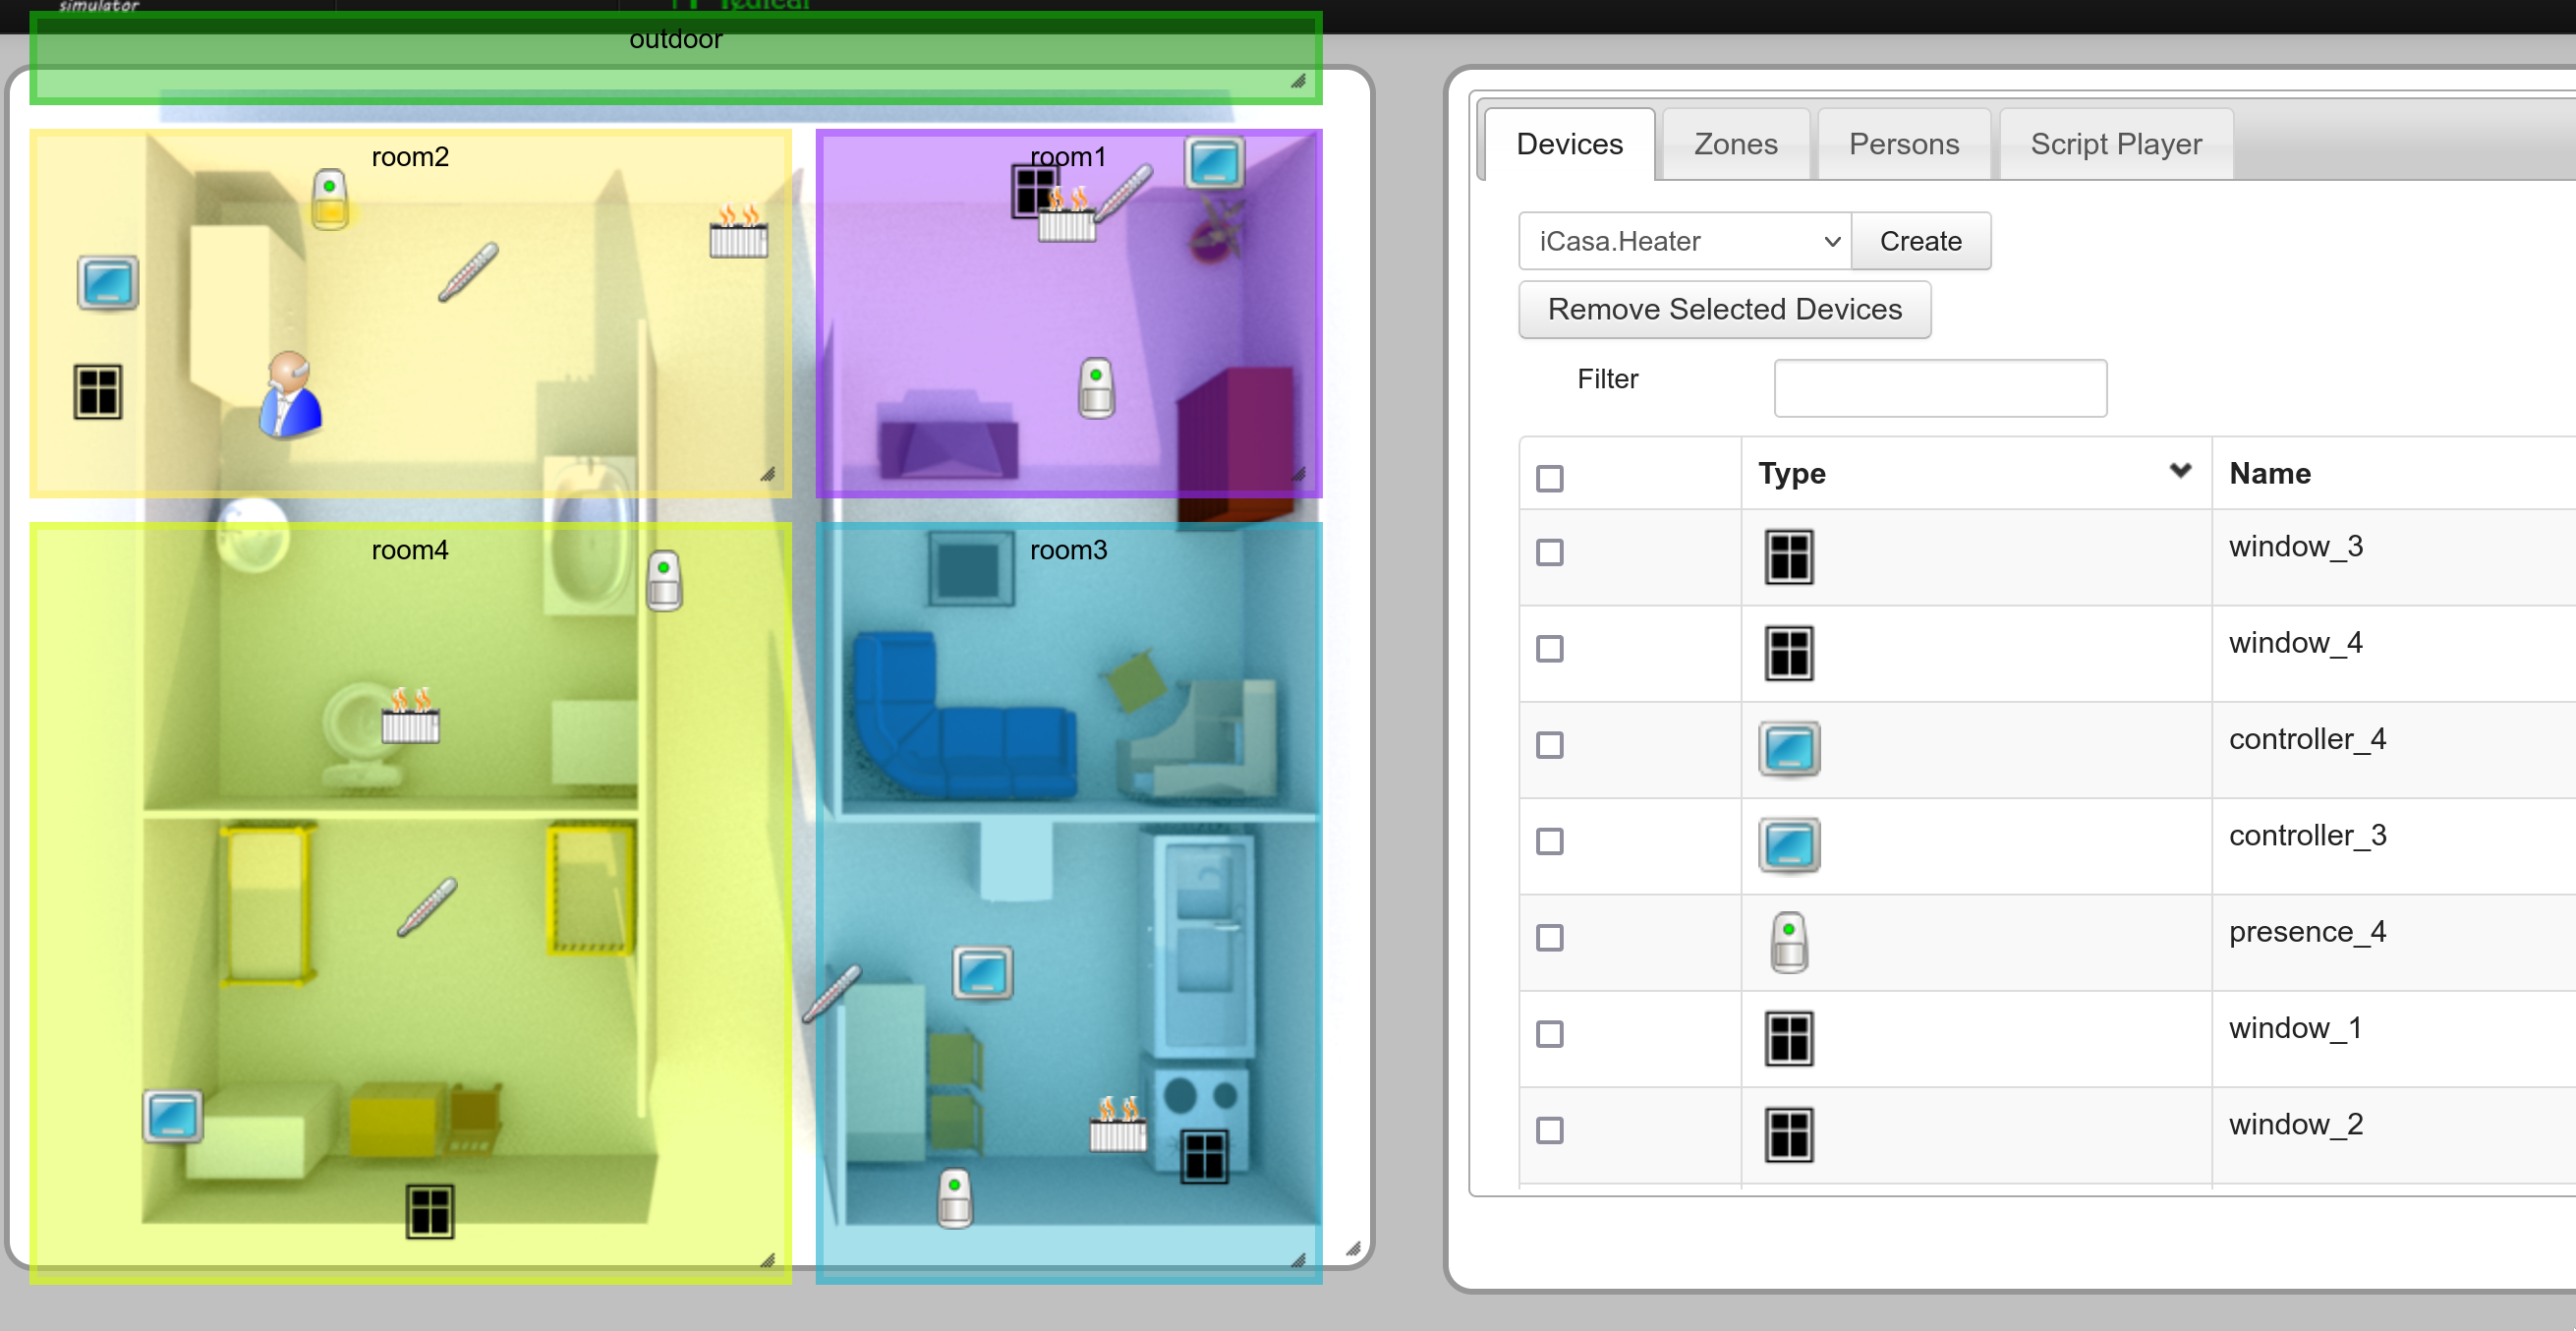
\includegraphics[width=\linewidth]{figures/simulator}
  \caption{View of the simulator's web interface provided by iCasa. The four rooms are visible, with their equipment and the user.}
  \label{fig:view}
\end{figure}

\begin{figure}[ht]
  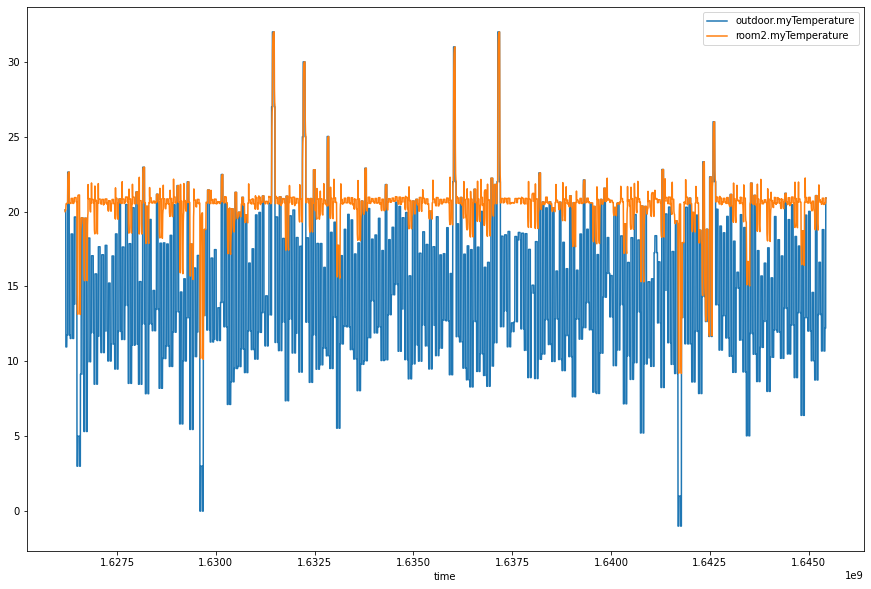
\includegraphics[width=\linewidth]{figures/ts_example}
  \caption{Time series data from the simulation: outdoor temperature and controller temperature of a room. We can see two temperature drops, one for each room. What could be the causes of these drops?}
  \label{fig:ts_example}
\end{figure}

The values of all devices and zones variables was regularly monitored throughout the simulation run, and the resulting data, which an excerpt is shown in figure \ref{fig:ts_exaple} can later be used as a basis for our experiments.
\subsection{Implementation}

For the implementation of our method, we first needed to identify and characterize events from the time series data generated by the iCasa simulation. Since this is not the focus point of our present work (see sec. \ref{sec:related}), we simply apply threshold and precomputed conditions based detections to create a base of events.


This base of events consists the basis of the initial memory $\mathcal{M}$ used for computations.

\subsection{Results}

\begin{figure}[ht]
  \centering
  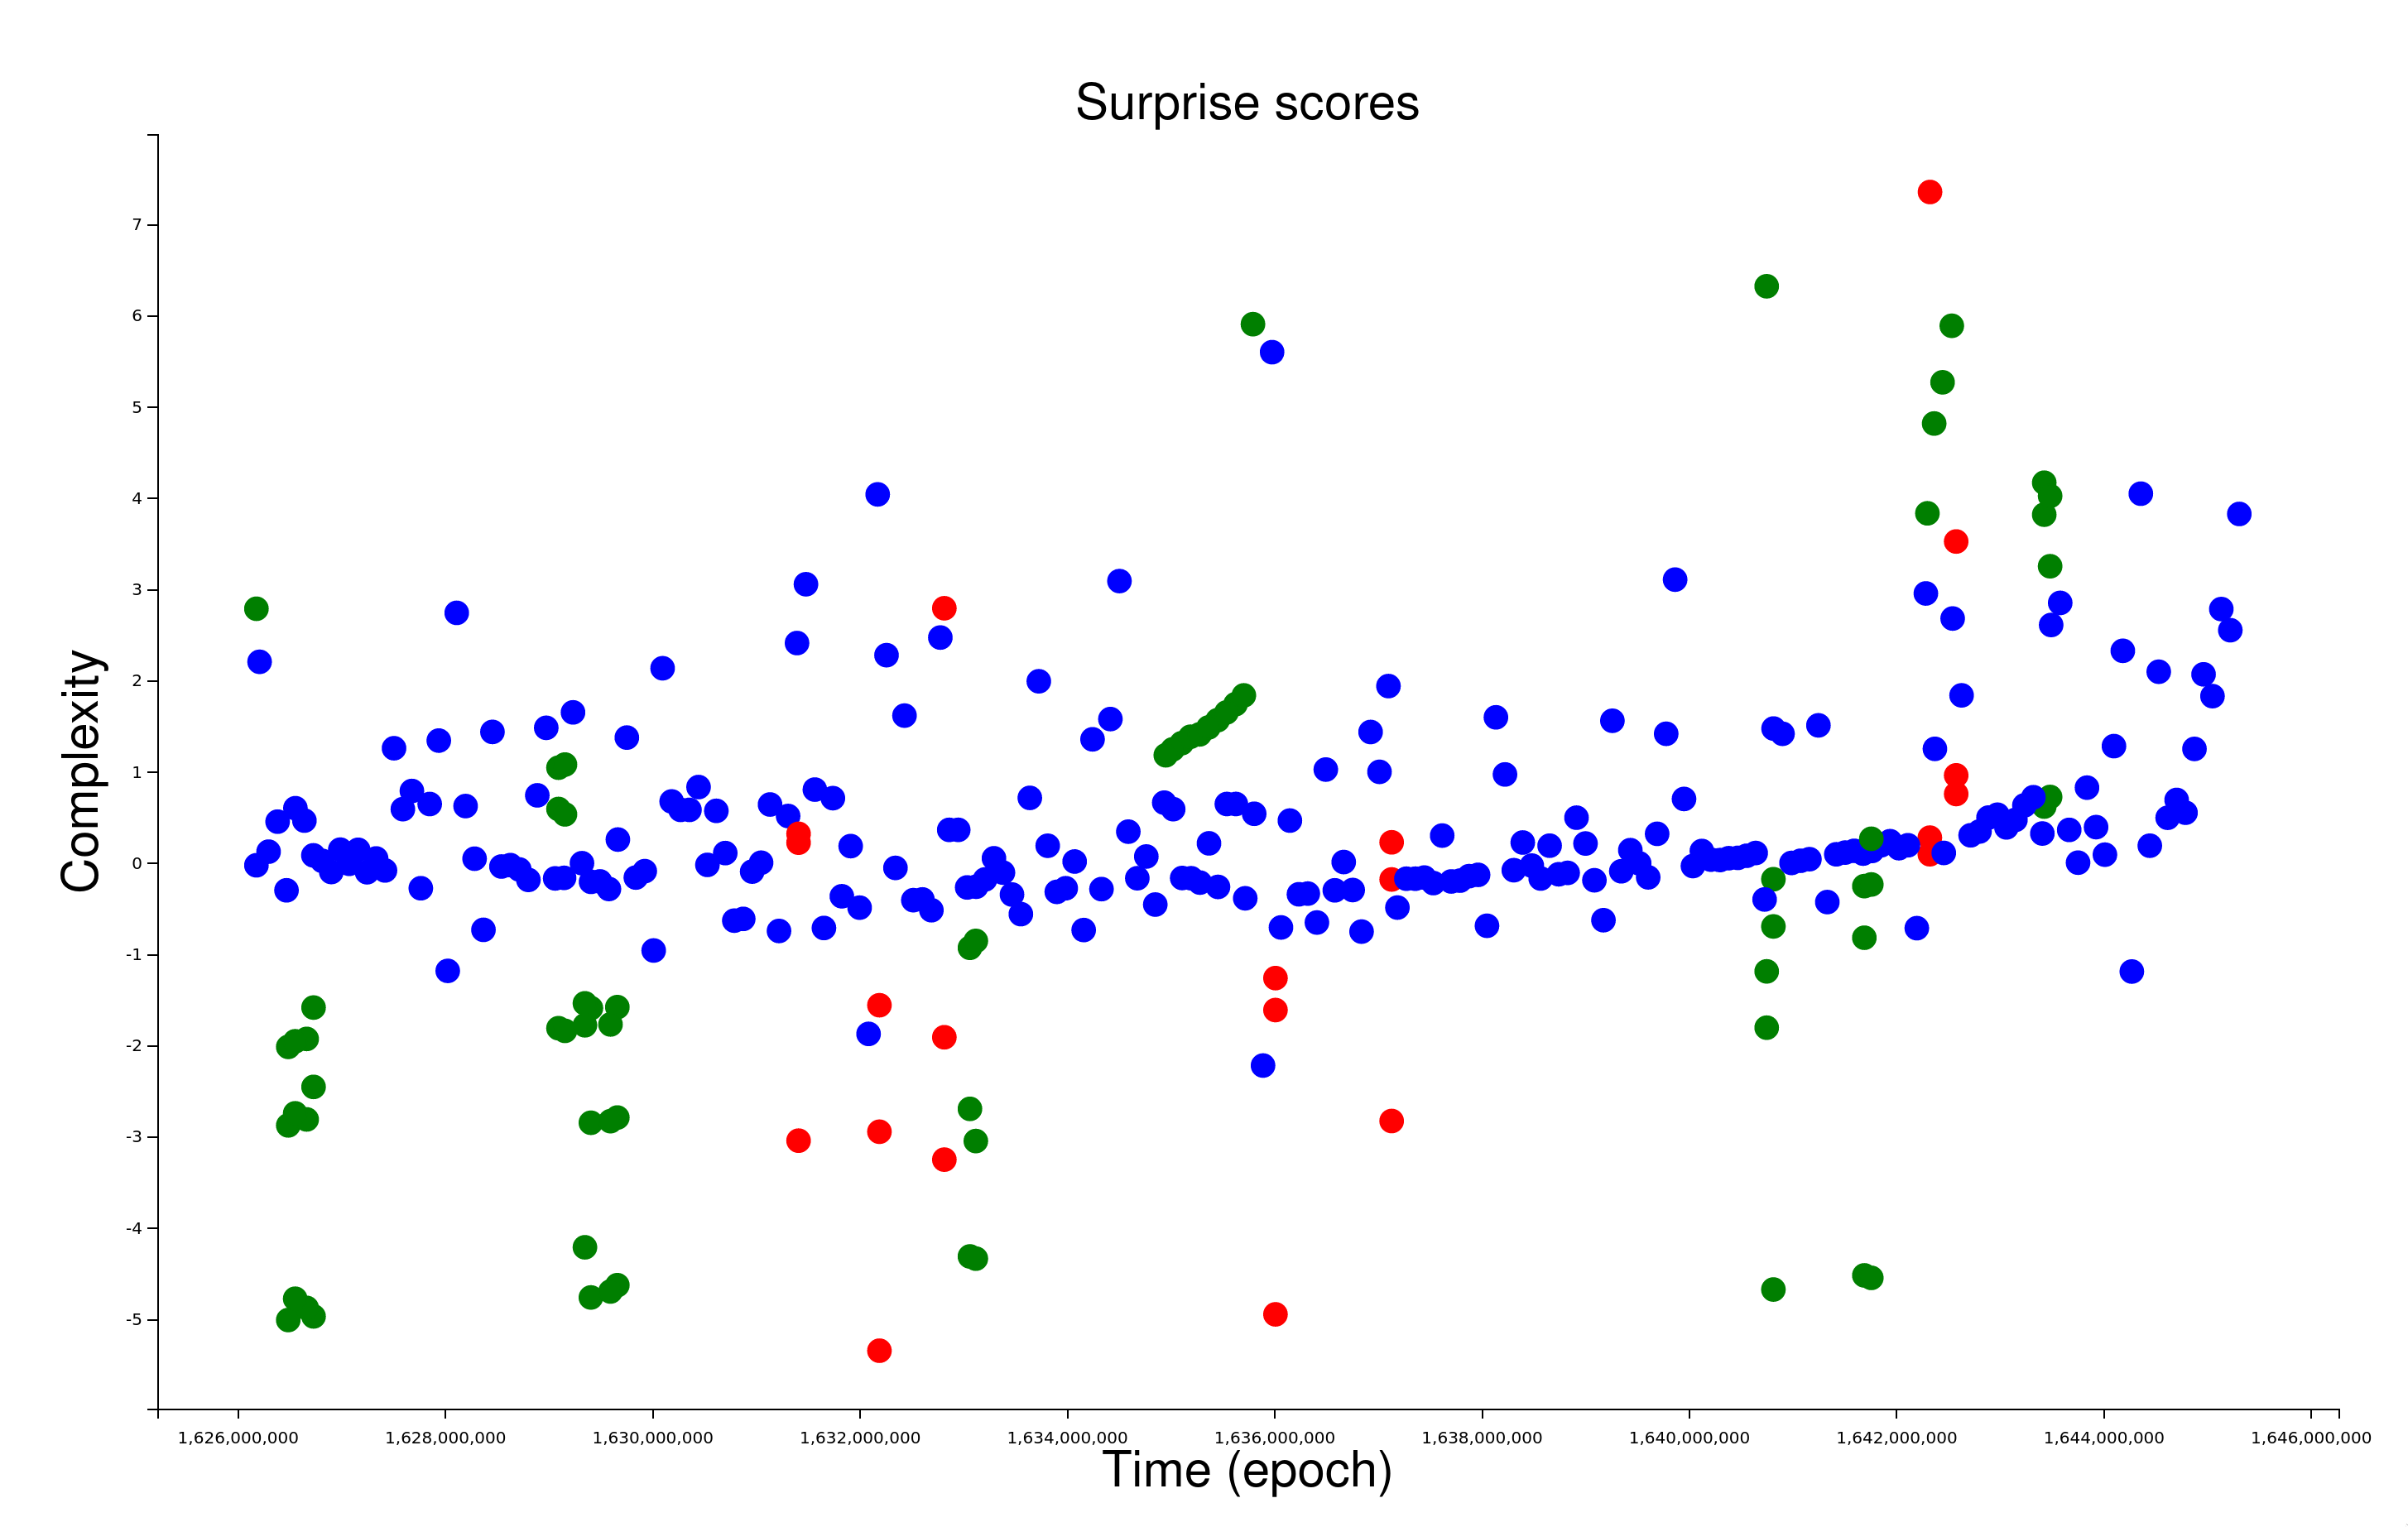
\includegraphics[width=\linewidth]{figures/surprises}
  \caption{Unnexpectedness score for events in the memory}
  \label{fig:result1}
\end{figure}

\section{Related Works}
\label{sec:related}

\section{Perspectives}

\section{Conclusion}


\bibliographystyle{IEEEtran}
\bibliography{biblio.bib}

\end{document}
